\chapter{Introduzione}
I microbi sono organismi unicellulari origine di tutte le forme di vita, mostrano una grande differenza tra di loro, maggiore di quella esistente tra piante
e animali, sono enormemente numerosi e ubiquitari. Trasformano e riciclano la materia organica e influenzano il clima. Hanno relaizoni simbiotiche con 
animali, piante e altri microorganismi. Alcuni sono patogeni. Possono sopravvivere a condizioni estreme:
\begin{itemize}
\item $5$ megarad di radiazioni gamma.
\item pH estremi: da $0$ a $11.4$.
\item Temperature estreme: da $-15$ a $121$ gradi centigradi.
\item Pressione idrostatica di $1300$ ATM.
\item Pressione osmotica corrispondente a $5.2$ di NaCl.
\end{itemize}
Si trovano sulla terra da molto prima della nascita di organismi pluricellulari. 
\section{Albero della vita}
\begin{figure}[h]
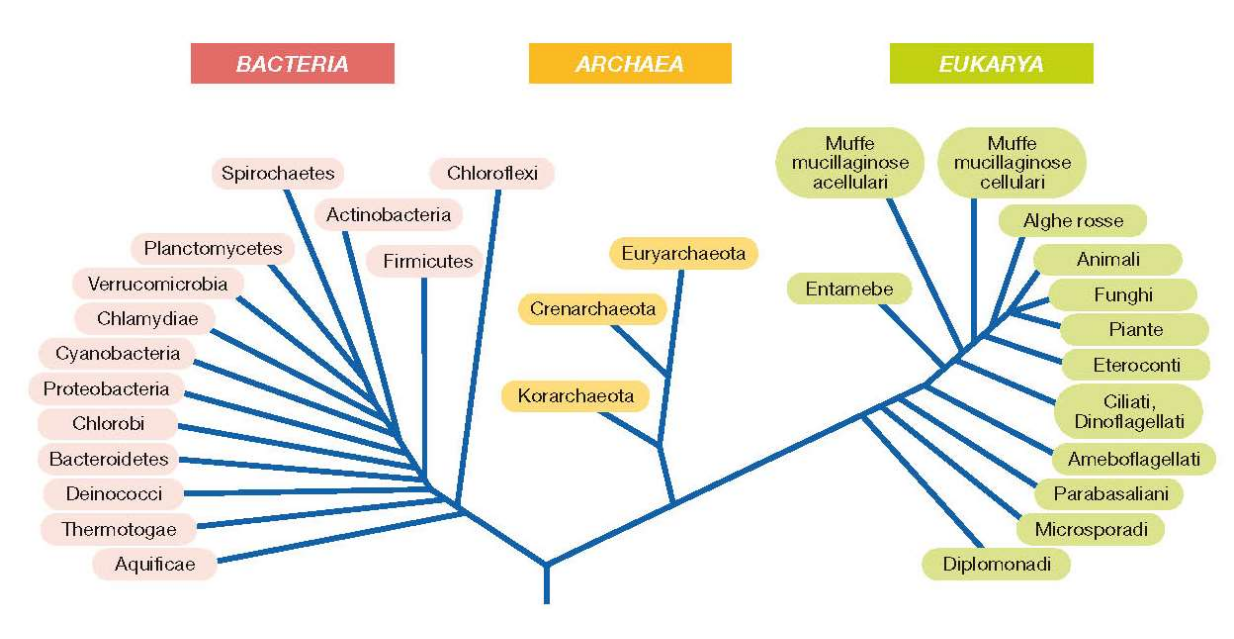
\includegraphics[width=\textwidth]{Pictures/AlberoVita.png}
\caption{Albero della vita}
\end{figure}
Oltre all'evoluzione in verticale nell'albero della vita possono accadere degli scambi in orizzontale tra specie molto distanti tra di loro. 
\subsection{Batteri e archei}
Batteri e archei sono organismi procarioti, ovvero non hanno nucleo cellulare, possiedono una parete cellulare polisaccarida di peptidoglicano. Svolgono una
riproduzione asessuata e sono tipicamente dalle 10 alle 100 volte pi\`u piccoli delle cellule eucariote, nell'ordine dei micrometri. 
\subsection{Virus}
I virus sono acellulari e costituiti da un materiale genetico a DNA o RNA, di un capside proteico e eventualmente di un ulteriore strato lipidico. Dipendono
dalla cellula ospite per la loro riproduzione. 
\subsection{Caratterizzazione dei microbi}
\begin{tabular}{|c|c|c|c|}
\hline
& Individuo & Popolazione & Comunit\`a \\
\hline
Ecologia & \makecell{Fisiologia:\\ differente espresisone\\ di geni in risposta\\ a cambiamenti} & \makecell{Demografica:\\ nascita, morte,\\ immigrazione, 
emigrazione} & \makecell{Ecologia comunitaria:\\ interazioni interspecie che \\danno forma a struttura e\\ funzione della comunit\`a}\\
\hline
Genomica & \makecell{Mappatura fine\\ di singoli genomi} & \makecell{Genomica della popolazione:\\ analisi genomica comparativa\\ per determinare 
variazioni} & \makecell{Metagenomica:\\ potenziale genetico \\dei membri della comunit\`a}\\
\hline
Genetica & \makecell{Genetica dei batteri:\\ ruolo dei geni\\ sotto certe variazioni} & \makecell{Genetica della popolazione:\\ frequenza della 
distribuzione\\ degli alleli} & \makecell{Genetica comunitaria:\\ interazione tra la composizione\\ genetica della comunit\`a e le\\ propriet\`a della \\
comunit\`a ecologica}\\
\hline
\end{tabular}
\section{La macchina cellulare}
Le condizioni necessarie affinch\`e la cellula possa riprodursi comprendono un adeguato supporto energetico e la presenza di precursori per la sintesi di 
nuove macromolecole. Le istruzioni codificate nel genoma devono essere replicate in modo che ogni cellula figlia possa riceverne una copia. Infine i geni
devono essere espressi attraverso trascrizione e traduzione per formare le proteine e le macromolecole necessarie per dare origine a una nuova cellula.
\begin{figure}[h]
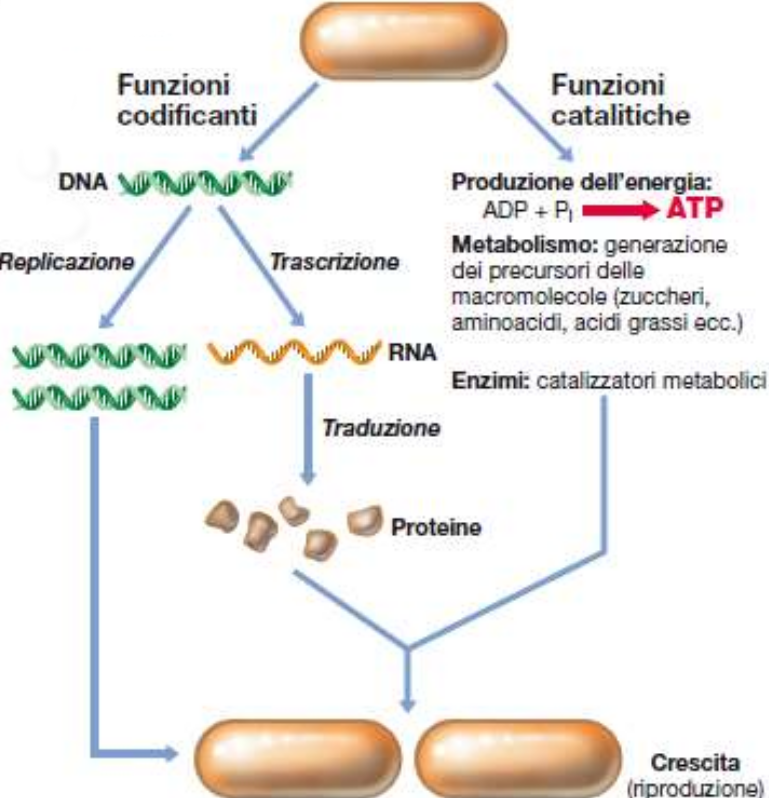
\includegraphics{Pictures/MacchinaCellulare.png}
\caption{Funzioni codificanti della macchina cellulare}
\end{figure}
\subsection{Impatto dei microbi sulle attivit\`a umane}
I microbi svolgono un ruolo fondamentale in varie attivit\`a umane:
\begin{itemize}
\item Agricoltura: fissazione di $N_2$ ($N_2\rightarrow 2NH_3$), necessario per il ciclo dei nutrienti, permettono ai ruminanti di consumare erba.
\item Cibo: preservazione del cibo, creazione di cibi fermentati e additivi.
\item Alcuni sono agenti patogeni.
\item Creazione di biofuels, bioremediation nel caso di petrolio disperso nell'ambiente e microbial mining.
\item Biotecnologie: produzione di organismi geneticamente modificati, produzione di prodotti farmaceutici, terapia genetia per certe malattie. 
\end{itemize}
\subsection{Ricombinazione del DNA}
I microbi sono utilizzati per ricombinare il DNA. Il DNA plasmidico e quello del donatore possono essere tagliati attraverso un'endonucleasi di restrizione
in modo da ottenere frammenti compatibili. Mescolando e legando il plasmide linearizzato il il DNA estraneo digerito i frammenti sono incorporati nel 
plasmide formando un plasmide ricombinante che viene inserito in cellule batteriche. Quando si riproduce viene riprodotto anche il DNA estraneo. Se il 
donatore contiene un gene questo pu\`o essere espresso producendo una proteina eterologa. 
\section{Microrganismi come modello}
I microrganismi sono stati ampiamente utilizzati per la ricerca in quanto si replicano velocemente, sono economici da coltivare e hanno strutture 
relativametne semplici. Sono stati pertanto utilizzati per studiare i processi cellulari come replicazione del DNA, trascrizione e traduzione. 
\subsection{Il conflitto sulla generazione spontanea}
Fino all'esperimento di Redi si credeva che gli organismi viventi potessero svilupparsi da matera non vivente o in decomposizione. Questa teoria viene
confutata ponendo della carne in putrefazione in tre vasi: uno scoperto (con conseguenza di deposito di larve di mosca), uno sigillato (che rimase senza 
larve) e uno coperto da una garza (su cui le mosche, attratte dall'odore deposero le larve).
\subsection{Postulati di Koch}
\begin{enumerate}
\item Il microrganismo deve essere presente in tutti gli individui affetti dalla malattia e assente in quelli sani.
\item Il microrganismo deve essere isolato dall'individuo affetto e, posto in coltura, deve dare origine a una popolazione cellulare omogenea.
\item L'inoculo di una cultura pura del microrganismo in individui sani pu\`o causare la comparsa della malattia di cui \`e ritenuto responsabile. 
\item Il microrganismo deve essere reisolato dall'organismo infetto sperimentalmente in cui la malattia sia insorta.
\end{enumerate}
\subsubsection{I postulati di Koch molecolari}
\begin{enumerate}
\item Il gene implicato nella patogenicit\`a o virulenza deve trovarsi in tutti i ceppi patogeni di una data specie ed essere assente dalle specie non 
patogene.
\item L'inattivazione selettiva del gene deve portare a una diminuzione misurabile della patogenicit\`a o virulenza.
\item La complementazione o reversione della mutazione deve ripristinare il livello originale di patogenicit\`a o virulenza. Parimenti l'introduizone del
gene in un ceppo non patogeno lo trasforma in patogeno.
\end{enumerate}